\chapter{La piattaforma robot}
\vspace{0.5cm}

\label{cha:789}
EvoBot unisce elementi dell'open source delle stampanti 3D e della robotica modulare per fornire a chimici, microbiologi e ricercatori nel campo della vita artificiale, a livello chimico, uno strumento economico ed estendibile basato su una piattaforma robotica open source per il trattamento di liquidi.
\\ La particolarità di Evobot sta nella progettazione mirata ad una interazione continua ed in tempo reale dell'utente con l'esperimento in corso.\cite{introd-robot}
\\La struttura di EvoBot ricorda quella di una comune stampante 3D, organizzata in strati.



\section{La componente hardware}
\label{sec:456}
EvoBot si compone, a livello meccanico, di tre strati ed è sotto il controllo di una \emph{board}. Questa è costituita da un Arduino Mega 2560 su cui è montata una scheda RAMPS (RepRap Arduino Mega Pololu Shield). Queste due schede controllano la testa del robot e gli input provenienti dai sensori esterni. 
Il primo dei tre strati mostrato in figura, è lo strato di attivazione, \emph{actuation layer}. 
	\begin{center}
	  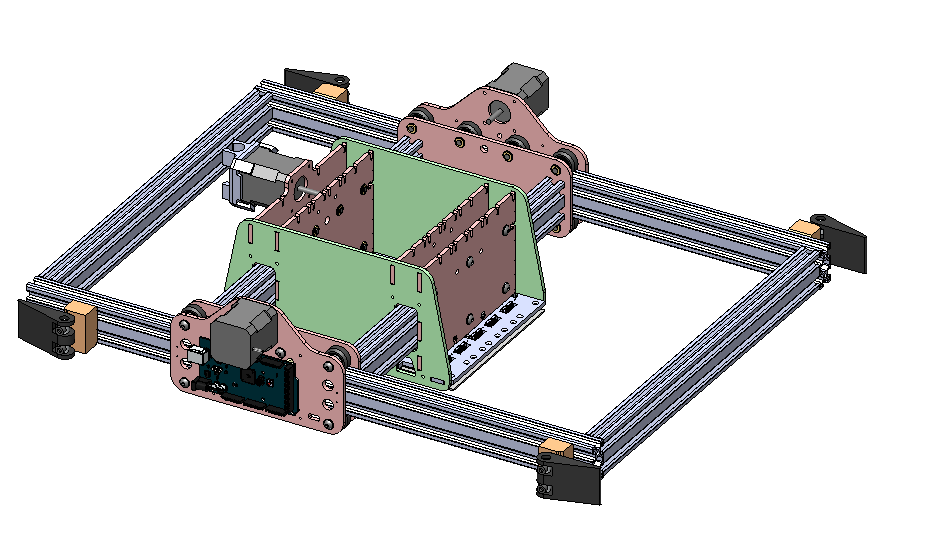
\includegraphics[scale=0.40]{actuation_layer.png}
	 %\caption{actuation layer}
	\end{center}
Questo contiene la testa che si può muovere sul piano orizzontale usando una cinghia ed un meccanismo a ruota dentata con due motori \emph{stepper}.
\\Il secondo strato è quello degli esperimenti: \emph{experimental layer}.
	\begin{center}
	  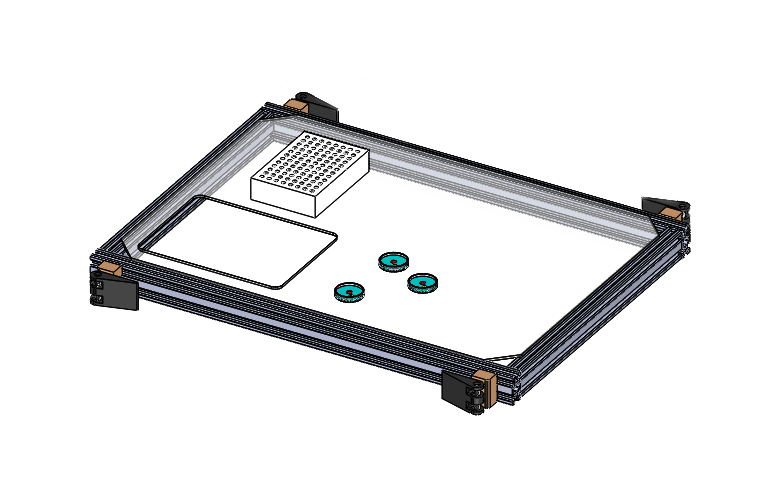
\includegraphics[scale=0.60]{experiment_layer.png}
	 %\caption{experimental layer}
	\end{center} 
Questo strato è essenzialmente composto da una cornice in alluminio, identica a quella della struttura esterna del robot, che racchiude una piastra di vetro trasparente. Su questo strato posso essere adagiati i recipienti richiesti dagli specifici esperimenti. Una fessura rettangolare ad uno degli angoli permette le manovre di sostituzione dei recipienti in uso. La sua funzionalità verrà sfruttata in futuro creando un distributore automatico di  \emph{Petri dish} da posizionarvi all'interno. 
L'ultimo strato è quello dell'osservazione: \emph{observation layer} .

\subsection{La testa}
\label{sec:00456}
La \emph{head}, testa del robot, è la componente principale dell'\emph{actuation layer}. Essa può contenere fino ad un massimo di 11 moduli per fornire funzionalità differenti. Ad oggi è stato implementato soltanto il modulo per le siringhe ma si prevede l'implementazione futura di altri moduli, sensori di pH, di temperatura e pinze per la manipolazione delle capsule di Petri utilizzate durante gli esperimenti. 
\\ La testa si può muovere in due direzioni sul livello orizzontale: gli assi \emph{x} e \emph{z}. Le schede che compongono la testa permettono di rispondere a stimoli esterni (?)
ramps . arduino

\subsection{Le siringhe}
\label{sec:01456}
come si fa un sottocapitolo

\section{La componente software}
\label{sec:123}
scrivere qualcosa di introduzione

\begin{itemize}
  \item API 
  \item bitbucket
  \item calibrazione
  \item processi visuali - threshold 
\end{itemize}


